
\chapter{观察性研究中的匹配方法}\label{chapter::matching-obs}
 
匹配方法在实证研究中有着悠久的历史。W. Cochran与D. Rubin将其引入统计因果推断领域。\citet{cochran1973controlling}是一篇早期的综述性论文；\citet{rubin2006matched}则汇总了Rubin在此方向上的研究成果。
本章还将探讨\citet{abadie2006large, abadie2008failure, abadie2011bias}基于匹配估计量渐近分析所提出的现代理论成果。 

 

\section{一个简单的起点：大量的对照组单位}
\label{sec::ideal-matching-mpe}

\begin{figure}[ht]
\centering 
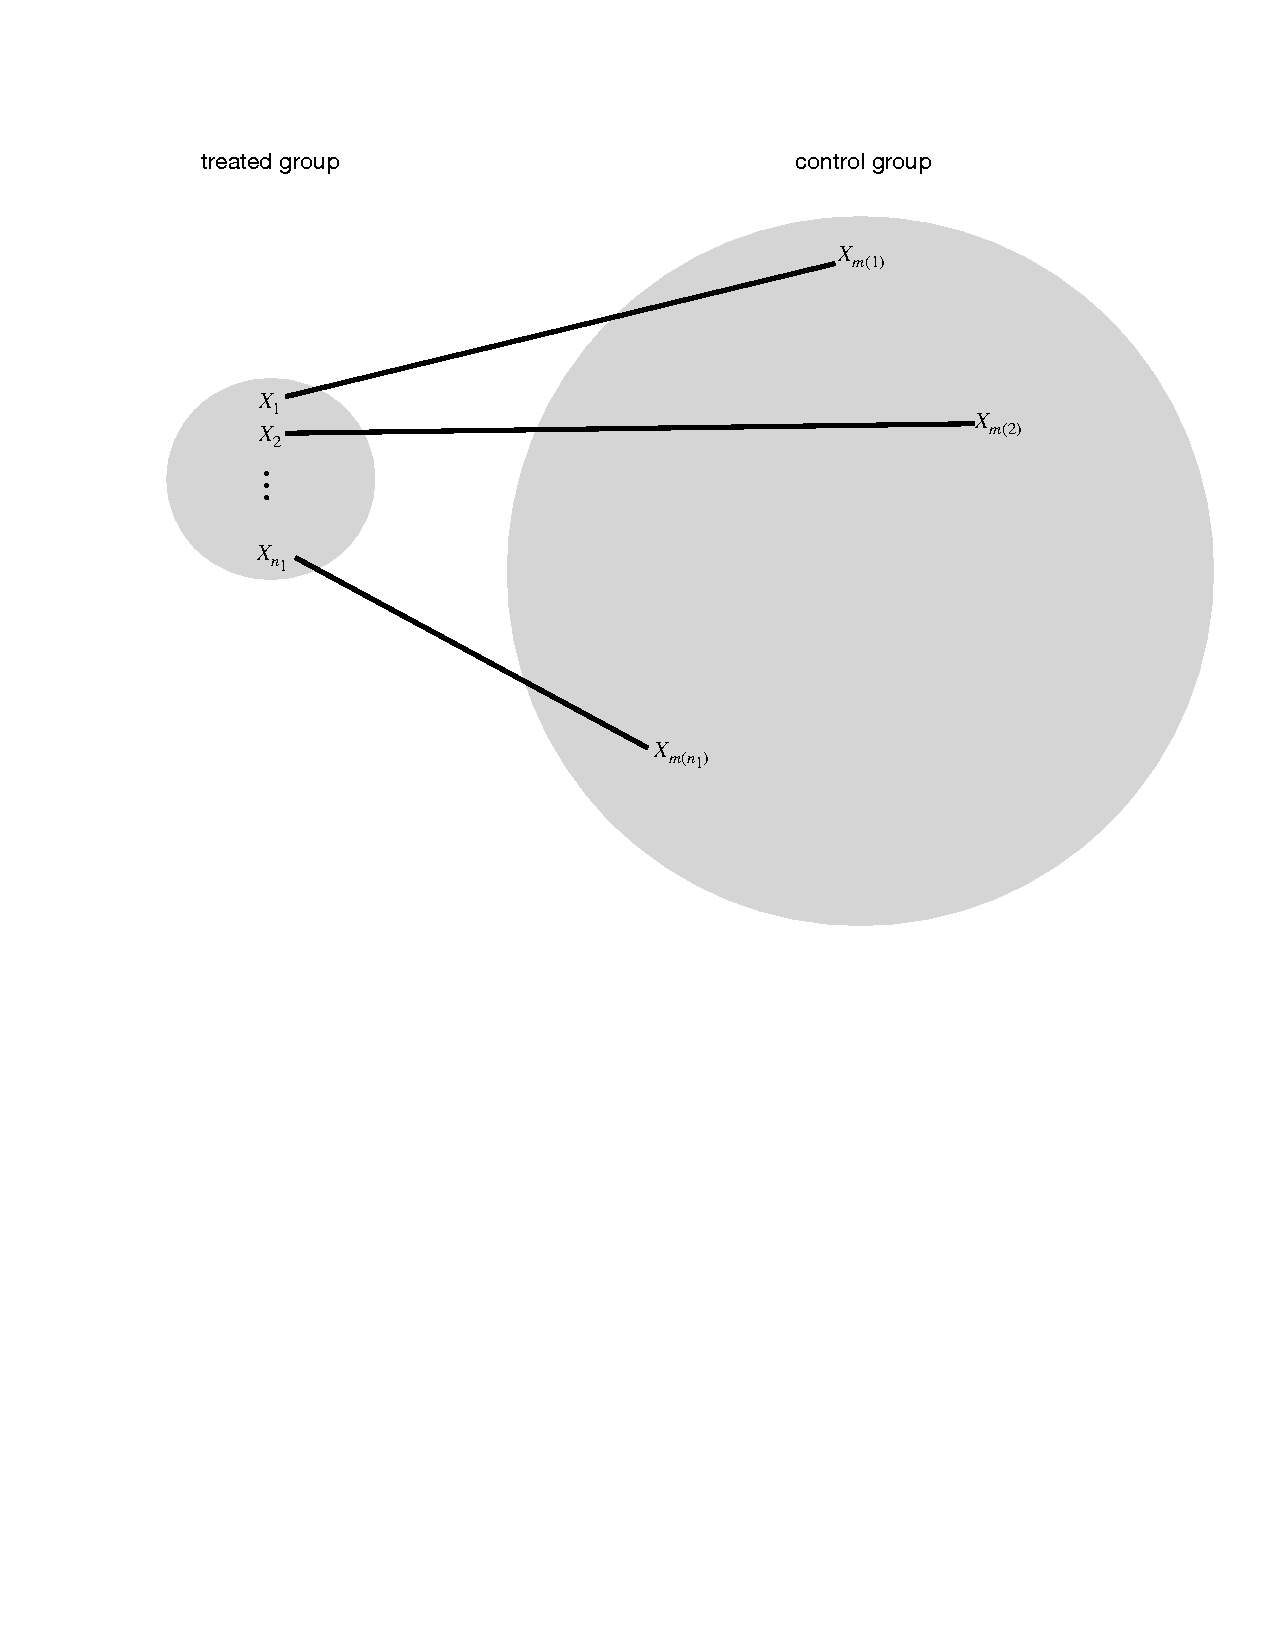
\includegraphics[width = \textwidth]{figures/matchingonetoone.pdf}
\caption{观察性研究中匹配方法的示意图}\label{fig::matching-causal}
\end{figure}


图\ref{fig::matching-causal}展示了处理—对照观察性研究中匹配的基本思想。考虑对照单位数$n_0$远大于处理单位数$ n_1$的简单情形。对处理组中的单位$i=1,\ldots, n_1$，在对照组中找到单位$m(i)$，使$X_i = X_{m(i)}$。理想情况下可以精确匹配，因此每个匹配对内两单位的倾向得分相同，即$e(X_i) = e(X_{m(i)})$。由对称性，在一单位接受处理、另一单位接受对照的条件下，单位$i$接受处理且单位$m(i)$接受对照的概率为$$
\pr( Z_i = 1, Z_{m(i)} = 0 \mid  Z_i +Z_{m(i)} = 1, X_i, X_{m(i)} )  = 1/2
$$\footnote{严格论证如下：\begin{eqnarray*}
&&\pr( Z_i = 1, Z_{m(i)} = 0 \mid  Z_i +Z_{m(i)} = 1, X_i, X_{m(i)} ) \\
&=& \frac{ \pr( Z_i = 1, Z_{m(i)} = 0 \mid   X_i, X_{m(i)} ) }{ \pr( Z_i = 1, Z_{m(i)} = 0 \mid   X_i, X_{m(i)} )   + \pr( Z_i = 0, Z_{m(i)} = 1 \mid   X_i, X_{m(i)} ) } \\
&=& \frac{  e(X_i)  \{ 1 - e(X_{m(i)}) \}  }{ e(X_i)  \{ 1 - e(X_{m(i)}) \}   + \{1-e(X_i)\} e(X_{m(i)}) } \\
&=& \frac{1}{2}.
\end{eqnarray*}}也就是说，给定协变量，并以每对恰有一处理单位和一对照单位为条件，处理分配机制与配对实验相同。因此，可以将精确匹配的观察性研究视为配对实验，用第\ref{chapter::mpe}章的FRT或内曼方法分析，推断已处理单位的因果效应。 


也可以为每个处理单位寻找多个对照单位。一般地，为处理单位$i$找到$M_i$个匹配的对照单位。当各个$M_i$不同时，称为{\it 变比例匹配}\citep{ming2000substantial, ming2001note, pimentel2015variable}。若匹配完全精确，处理分配机制就与第\ref{sec::general-matched-experiment}节讨论的一般匹配实验相同，可以用该节的解析结果分析匹配后的观察性研究。 


\citet{rosenbaum2002design}倡导了上述分析思路。然而在多数观察性研究中，$X_i = X_{m(i)}$这个条件往往无法满足所有单位。此时前述FRT分析逻辑不再成立。最近，\citet{guo2022statistical}指出了不完全匹配情形下FRT方法存在的负面效应，这也为该分析策略敲响了警钟。 
 


\section{更为复杂但更现实的情形}

即便对照组单位数量众多，我们也往往难以实现完全匹配。此时我们只能保证在某种距离度量下$X_i \approx X_{m(i)}  $或$X_i -X_{m(i)} $的值较小。也就是说我们只能获得近似匹配结果。例如，我们可定义
$$
m(i) = \arg\min_{k:Z_k = 0} d(X_i ,X_k), 
$$
其中$d(X_i ,X_k)$表示$X_i$与$X_k$之间的距离。常见的距离度量方式包括欧几里得距离
$$
d(X_i ,X_k) =  (X_i - X_k)\tran ( X_i - X_k),
$$
以及马氏距离
%\footnote{We define $\|v\|_2^2 = \sum_{j=1}^p v_j^2$ for a vector $v = (v_1, \ldots, v_p)\tran$. It denotes the squared length of the vector $v$.}
$$
d(X_i ,X_k) =(X_i - X_k)\tran \Omega^{-1} (X_i - X_k)
$$
此处$\Omega$为总体或对照组单位$X_i$的样本协方差矩阵。 


下文将探讨与匹配方法相关的若干细节问题。相关综述文献可参见\citet{stuart2010matching}。 
\begin{enumerate}
\item
（一对一或一对$M$匹配）
前述讨论均基于一对一匹配方式，上述逻辑亦可推广至一对$M$匹配情形。


\item
本文主要讨论有放回匹配方式，但也有研究者偏好无放回匹配。当对照组单位数量庞大时，这两种方式对最终分析结果的影响通常不大。有放回匹配计算方便，但无放回匹配则涉及复杂的离散最优化计算。有放回匹配所得匹配对质量通常更高，然而因同一单位可能多次参与匹配而带来单位间相关性问题。反之，无放回匹配的优势在于匹配单位间相互独立且后续数据分析更为简便。 


\item
由于匹配过程中配对单位间仍可能存在协变量不均衡问题，因此数据分析时必须进行协变量调整。此时协变量调整不仅为提升估计效率，更是为了纠正潜在偏差。

\item
如果$X$是高维的，那么可能对某个处理单位$i$而言，无论选择哪个对照单位，$d(X_i ,X_k)$都过大。此时可能不得不舍弃一些难以匹配的单位。这样做实际上改变了研究所针对的总体。  


\item
上述问题很难避免。例如，若$X_i \sim \text{N}(0, I_p), X_k \sim\text{N}(0, I_p) ,$且$X_i \ind X_k$，则$$
(X_i - X_k)\tran (X_i - X_k) \sim    2 \chi^2_p
$$其均值为$2p$、方差为$8p$，见第\ref{subsection::chi2-t-distribution}章。理论表明，$p$较大时，不精确匹配会使因果效应估计产生较大偏差。因此，若$p$较大，应在匹配前进行降维。\citet{rosenbaum1983central}提出根据倾向得分匹配。利用估计倾向得分，寻找单位对$\{ i, m(i)\}$，使$ |  \hat{e}(X_i) -  \hat{e}(X_{m(i)})  |$或$| \logit\{ \hat{e}(X_i)\} - \logit\{ \hat{e}(X_{m(i)}) \} | $较小\footnote{定义$\logit(w) = \log \frac{w}{1-w}$。logit函数将$(0,1)$映射到$(-\infty, \infty)$。}，从而将问题化为一维匹配。 
\end{enumerate}

 

\section{平均因果效应的匹配估计量}

Abadie与Imbens（简称AI）通过一系列研究严谨地刻画了匹配估计量的渐近特性，并提出了针对平均因果效应的大样本置信区间计算方法。
他们的研究以观察性研究的经典模型为基准，即$\{ X_i , Z_i ,Y_i(1), Y_i(0)  \}_{i=1}^n \iidsim \{ X, Z, Y(1), Y(0) \}$。  

\subsection{点估计与偏差校正}

AI主要研究有放回的$1$对$M$匹配。对于处理单位$i$，处理下的潜在结果直接插补为$\hat{Y}_i(1) = Y_i$，对照下的潜在结果则插补为$$
\hat{Y}_i(0) = M^{-1} \sum_{k\in J_i} Y_k,
$$其中$J_i$是单位$i$在对照组中的匹配单位集合。例如，可以对所有对照单位$k$计算$d(X_i, X_k)$，再将$J_i$定义为使$d(X_i, X_k)$取最小$M$个值的单位$k$的下标集合。 




对于对照单位$i$，对照下的潜在结果直接插补为$\hat{Y}_i(0) = Y_i$，处理下的潜在结果则插补为$$
\hat{Y}_i(1) = M^{-1} \sum_{k\in J_i} Y_k,
$$其中$J_i$是单位$i$在处理组中的匹配单位集合。

最终匹配估计量定义为
$$
\hat{\tau}^\textup{m} = n^{-1} \sumn \{\hat{Y}_i(1) -\hat{Y}_i(0) \}.
$$

AI证明，$\hat{\tau}^\textup{m}$的偏差不可忽略，尤其是在$X$为多维、且对照单位数与处理单位数相近时。经过技术推导，他们提出以下偏差估计量：$$
\hat{B} = n^{-1} \sumn  \hat{B}_i
$$其中$$
\hat{B}_i = (2Z_i - 1) M^{-1} \sum_{k\in J_i} \{  \hat{\mu}_{1-Z_i}(X_i) -  \hat{\mu}_{1-Z_i}(X_k)     \}
$$$\{  \hat{\mu}_1(X_i), \hat{\mu}_0(X_i) \}$为例如通过OLS拟合得到的结果预测值。对于满足$Z_i  =1$的处理单位，估计偏差为$$
\hat{B}_i = M^{-1} \sum_{k\in J_i} \{  \hat{\mu}_{0}(X_i) -  \hat{\mu}_{0}(X_k)     \}
$$用于修正协变量不匹配导致的对照潜在结果预测差异；对于满足$Z_i = 0$的对照单位，估计偏差为$$
\hat{B}_i =  - M^{-1} \sum_{k\in J_i} \{  \hat{\mu}_{1}(X_i) -  \hat{\mu}_{1}(X_k)     \}
$$用于修正协变量不匹配导致的处理潜在结果预测差异。 


最终经偏差校正后的匹配估计量为
$$
\hat{\tau}^\textup{mbc} = \hat{\tau}^\textup{m}  - \hat{B},
$$
它具有如下线性展开形式。
 
 \begin{proposition}
 \label{prop::matching-expansion-ate} 我们有 
\begin{eqnarray}\label{eq::linearATE}
\hat{\tau}^\textup{mbc}  
= n^{-1} \sumn \hat{\psi}_i
\end{eqnarray} 
其中 
$$
  \hat{\psi}_i = \hat{\mu}_1(X_i) -  \hat{\mu}_0(X_i) + (2Z_i - 1) (1+K_i/M) \{   Y_i - \hat{\mu}_{Z_i}(X_i)  \}
 $$
$K_i$为单位$i$被选作匹配对象的次数。 
 \end{proposition}
 
 
 
命题\ref{prop::matching-expansion-ate}中的线性展开可以通过简单但繁琐的代数运算得到，其证明留作习题\ref{para::linear-bcm-ate}。将$\hat{\tau}^\textup{mbc}  $看作各$  \hat{\psi}_i $的样本均值，便可由线性展开得到简单的方差估计量$$
\hat{V}^\textup{mbc}  = \frac{1}{n^2} \sumn (  \hat{\psi}_i - \hat{\tau}^\textup{mbc}  )^2,
$$\citet{abadie2008failure}首先指出，对原始数据直接进行重抽样的普通自助法不能正确估计匹配估计量的方差，但他们提出的方差估计程序不易实现。\citet{otsu2017bootstrap}提出对线性展开中的$  \hat{\psi}_i $进行自助抽样。然而，\citet{otsu2017bootstrap}的自助法实质上给出的就是易于计算的方差估计量$\hat{V}^\textup{mbc}  $。 


 
\subsection{与双重稳健估计量的关系}
 \label{sec::connection-dr-att}
 
偏差修正匹配估计量与双重稳健估计量密切相关。两者都是在结果回归估计量上，根据残差作某种修正：$$ 
 \hat{R}_i = 
 \begin{cases}
 Y_i - \hat{\mu}_1(X_i)  & \text{ if } Z_i=1;\\
 Y_i - \hat{\mu}_0(X_i)    & \text{ if } Z_i=0.
\end{cases} 
 $$对于平均因果效应$\tau$，回顾结果回归估计量$$
\hat{\tau}^{\textup{reg}} =  n^{-1} \sumn \{ \hat{\mu}_1(X_i) -  \hat{\mu}_0(X_i)\} 
$$和双重稳健估计量$$
\hat{\tau}^\textup{dr}  =  \hat{\tau}^{\textup{reg}} 
+ n^{-1} \sumn \left\{  \frac{Z_i \hat{R}_i }{ \hat{e}(X_i)} -  \frac{ (1-Z_i) \hat{R}_i}{ 1-  \hat{e}(X_i) } \right\} .
$$进一步可以验证，$\hat{\tau}^\textup{mbc} $具有与$\hat{\tau}^\textup{dr}  $相似的形式。
\begin{proposition}
\label{prop::mbc-dr}
经偏差校正后的$\tau$匹配估计量可表示为
$$
\hat{\tau}^\textup{mbc}   =\hat{\tau}^{\textup{reg}} 
+ n^{-1} \sumn \left\{ \left(1+{ K_i\over M} \right)  Z_i \hat{R}_i  - \left( 1+{ K_i\over M} \right) (1-Z_i)  \hat{R}_i \right\} .
$$
\end{proposition}

命题\ref{prop::mbc-dr}的证明留作习题\ref{para::dr-mbc-form}。由命题\ref{prop::mbc-dr}可将匹配看作估计倾向得分的一种非参数方法，并将相应的偏差修正匹配估计量看作双重稳健估计量。例如，$1+K_i /  M$应接近$1/\hat{e}(X_i)$。若某处理单位的$e(X_i)$较小，则基于估计倾向得分的权重$1/\hat{e}(X_i)$较大；同时，它会与很多对照单位匹配，使$K_i$以及$1+K_i /  M$也较大。不过，这种联系也引出了一个明显的问题：当$M$固定时，用$1+K_i /  M$估计$1/e(X_i)$的噪声很大。允许$M$随样本量增大，有望改善基于匹配的倾向得分非参数估计，进而改善匹配及偏差修正匹配估计量的渐近性质。\citet{lin2023estimation}给出了严格理论：只要$M$按适当速率增长，偏差修正匹配估计量$\hat{\tau}^\textup{mbc}   $就能达到与双重稳健估计量相似的性质。  


 
 
 \section{平均治疗效应匹配估计量的推导}

 
对于已处理单位的平均因果效应$$
\tau_\textsc{T} = E(Y\mid Z=1) - E\{  Y(0)  \mid Z=1\},
$$只需为所有处理单位插补缺失的对照潜在结果，即得估计量$$
\hat{\tau}_\textsc{T}^\textup{m} = n_1^{-1} \sumn Z_i \{  Y_i - \hat{Y}_i(0) \}.
$$当$X$为多维时，它同样存在偏差。\citet{otsu2017bootstrap}提出以下偏差估计量：$$  
\hat{B}_\textsc{T} = n_1^{-1} \sumn Z_i  \hat{B}_{\textsc{T},i} 
$$其中$$
\hat{B}_{\textsc{T},i} = M^{-1} \sum_{k \in J_i} \{  \hat{\mu}_0(X_i) -  \hat{\mu}_0(X_k)     \}
$$用于修正满足$Z_i = 1.$的处理单位因协变量不匹配而产生的偏差。


最终经偏差校正后的估计量为：
$$
\hat{\tau}_\textsc{T}^\textup{mbc} = \hat{\tau}_\textsc{T}^\textup{m} - \hat{B}_\textsc{T},
$$ 
其具有如下线性展开形式。

\begin{proposition}\label{prop::linear-expansion-att}
我们有 
\begin{eqnarray}\label{eq::linearATT}
\hat{\tau}_\textsc{T}^\textup{mbc}  =   n_1^{-1} \sumn \hat{\psi}_{\textsc{T}, i},
\end{eqnarray}
其中 
$$
\hat{\psi}_{\textsc{T}, i} =   Z_i \{ Y_i - \hat{\mu}_0(X_i) \}
- (1-Z_i) K_i/M \{ Y_i - \hat{\mu}_0(X_i) \} . 
$$
\end{proposition}

证明留作习题\ref{para::linear-bcm-ate}。受\citet{otsu2017bootstrap}启发，可以将$\hat{\tau}_\textsc{T}^\textup{mbc}  $看作$n/n_1$与各$\hat{\psi}_{\textsc{T}, i}$样本均值的乘积，因此一个直观的方差估计量为$$
\hat{V}_\textsc{T}^\textup{mbc} =  \left( \frac{n}{n_1} \right)^2 \frac{1}{n^2} \sumn (\hat{\psi}_{\textsc{T}, i} - \hat{\tau}_\textsc{T}^\textup{mbc} n_1/n)^2 = \frac{1}{n_1^2} \sumn (\hat{\psi}_{\textsc{T}, i} - \hat{\tau}_\textsc{T}^\textup{mbc} n_1/n )^2.
$$

 
 与第\ref{sec::connection-dr-att}节的讨论类似，可以将双重稳健估计量和偏差修正匹配估计量与结果回归估计量进行比较。对于已处理单位的平均因果效应$\tau_\textsc{T}$，回顾结果回归估计量$$
\hat{\tau}^{\textup{reg}}_\textsc{T} = n_1^{-1} \sumn Z_i \{ Y_i - \hat{\mu}_0(X_i) \} ,
$$和双重稳健估计量$$
\hat{\tau}_\textsc{T}^\textup{dr} =  \hat{\tau}^{\textup{reg}}_\textsc{T} 
- n_1^{-1} \sumn \frac{  \hat{e}(X_i) }{ 1- \hat{e}(X_i) }  (1-Z_i)  \hat{R}_i .
$$进一步可以验证，$\hat{\tau}_\textsc{T}^\textup{mbc} $具有与$\hat{\tau}_\textsc{T}^\textup{dr} $相似的形式。 
\begin{proposition}
\label{prop::mbc-dr-att}
经偏差校正后的$\tau_\textsc{T}$匹配估计量可表示为
$$
\hat{\tau}_\textsc{T}^\textup{mbc}   = \hat{\tau}^{\textup{reg}}_\textsc{T} 
 - n_1^{-1} \sumn { K_i\over M}  (1-Z_i)  \hat{R}_i.
$$
\end{proposition}


命题\ref{prop::mbc-dr-att}的证明留作习题\ref{para::dr-mbc-form-att}。命题\ref{prop::mbc-dr-att}表明，匹配实质上是用$K_i/M$估计给定协变量时接受处理的优势。 




\section{实例分析}
\label{sec::matching-application}



\subsection{实验数据}
现在使用\citet{sekhon2011multivariate}的\ri{Matching}包重新分析LaLonde数据。此前已多次使用该包中的\ri{lalonde}数据集，这里将使用其核心函数\ri{Match}。实验部分得到以下结果：
\begin{lstlisting}
> library("car")
> library("Matching")
> 
> ## Chapter 15.5.1
> ## experimental data
> data("lalonde")
> y = lalonde$re78
> z = lalonde$treat
> x = as.matrix(lalonde[, c("age", "educ", "black",
+                           "hisp", "married", "nodegr",
+                           "re74", "re75")])
> 
> ## analysis the randomized experiment
> neymanols = lm(y ~ z)
> fisherols = lm(y ~ z + x)
> xc = scale(x)
> linols = lm(y ~ z*xc)
> resols = c(neymanols$coef[2],
+            fisherols$coef[2],
+            linols$coef[2],
+            sqrt(hccm(neymanols, type = "hc2")[2, 2]),
+            sqrt(hccm(fisherols, type = "hc2")[2, 2]),
+            sqrt(hccm(linols, type = "hc2")[2, 2]))
> resols = matrix(resols, 3, 2)
> rownames(resols) = c("neyman", "fisher", "lin")
> colnames(resols) = c("est", "se")
> resols 
            est       se
neyman 1794.343 670.9967
fisher 1676.343 677.0493
lin    1621.584 694.7217
\end{lstlisting} 
各回归估计量均显示职业培训项目具有显著正向效应。若采用一对一匹配方式分析该实验数据，可得：
\begin{lstlisting}
> matchest.adj = Match(Y = y, Tr = z, X = x, BiasAdjust = TRUE)
> summary(matchest.adj)

Estimate...  2119.7 
AI SE......  876.42 
T-stat.....  2.4185 
p.val......  0.015583 

Original number of observations..............  445 
Original number of treated obs...............  185 
Matched number of observations...............  185 
Matched number of observations  (unweighted).  268
\end{lstlisting} 
估计值与标准误虽有所上升，但结论未发生改变。 


\subsection{观察性数据}
接着重新分析与上述实验相对应的观察性数据：
\begin{lstlisting}
> dat <- read.table("cps1re74.csv", header = TRUE)
> dat$u74 <- as.numeric(dat$re74==0)
> dat$u75 <- as.numeric(dat$re75==0)
> y = dat$re78
> z = dat$treat
> x = as.matrix(dat[, c("age", "educ", "black",
+                           "hispan", "married", "nodegree",
+                           "re74", "re75", "u74", "u75")])
 \end{lstlisting} 
然而采用一对一匹配方式后可得接近实验基准值的估计结果：
\begin{lstlisting}
> neymanols = lm(y ~ z)
> fisherols = lm(y ~ z + x)
> xc = scale(x)
> linols = lm(y ~ z*xc)
> resols = c(neymanols$coef[2],
+            fisherols$coef[2],
+            linols$coef[2],
+            sqrt(hccm(neymanols, type = "hc2")[2, 2]),
+            sqrt(hccm(fisherols, type = "hc2")[2, 2]),
+            sqrt(hccm(linols, type = "hc2")[2, 2]))
> resols = matrix(resols, 3, 2)
> rownames(resols) = c("neyman", "fisher", "lin")
> colnames(resols) = c("est", "se")
> resols 
             est        se
neyman -8506.495  583.4426
fisher  1067.546  628.4389
lin    -4265.801 3211.7718
  \end{lstlisting} 
  忽略匹配结果中的重复单位问题，采用配对分析方法可得到类似实验数据的结果：
  \begin{lstlisting}
> matchest = Match(Y = y, Tr = z, X = x, BiasAdjust = TRUE)
> summary(matchest)

Estimate...  1747.8 
AI SE......  916.59 
T-stat.....  1.9068 
p.val......  0.056543 

Original number of observations..............  16177 
Original number of treated obs...............  185 
Matched number of observations...............  185 
Matched number of observations  (unweighted).  248
   \end{lstlisting} 
   
忽略匹配数据中的并列匹配，还可以使用配对分析，其结果同样与实验数据的结果相近：
  \begin{lstlisting}
> diff = y[matchest$index.treated] - 
+           y[matchest$index.control]
> round(summary(lm(diff ~ 1))$coef[1, ], 2)
  Estimate Std. Error    t value   Pr(>|t|) 
   1581.44     558.55       2.83       0.01 
> 
> diff.x = x[matchest$index.treated, ] - 
+               x[matchest$index.control, ]
> round(summary(lm(diff ~ diff.x))$coef[1, ], 2)
  Estimate Std. Error    t value   Pr(>|t|) 
   1842.06     578.37       3.18       0.00 
   \end{lstlisting} 
   
   
   
   \subsection{协变量均衡性检验}
   
我们还可通过简单OLS检验匹配前后协变量分布。匹配前协变量存在严重不均衡性，具体表现为大量回归系数带有显著性标记。 
  \begin{lstlisting}
> lm.before = lm(z ~ x)
> summary(lm.before) 

Residuals:
     Min       1Q   Median       3Q      Max 
-0.18508 -0.01057  0.00303  0.01018  1.01355 

Coefficients:
              Estimate Std. Error t value Pr(>|t|)    
(Intercept)  1.404e-03  6.326e-03   0.222   0.8243    
xage        -4.043e-04  8.512e-05  -4.750 2.05e-06 ***
xeduc        3.220e-04  4.073e-04   0.790   0.4293    
xblack       1.070e-01  2.902e-03  36.871  < 2e-16 ***
xhispan      6.377e-03  3.103e-03   2.055   0.0399 *  
xmarried    -1.525e-02  2.023e-03  -7.537 5.06e-14 ***
xnodegree    1.345e-02  2.523e-03   5.331 9.89e-08 ***
xre74        7.601e-07  1.806e-07   4.208 2.59e-05 ***
xre75       -1.231e-07  1.829e-07  -0.673   0.5011    
xu74         4.224e-02  3.271e-03  12.914  < 2e-16 ***
xu75         2.424e-02  3.399e-03   7.133 1.02e-12 *** 
      \end{lstlisting} 
      
      
      匹配后所有回归系数均不再具有显著性标记，表明协变量分布已显著均衡。 
      
      
   \begin{lstlisting}
> lm.after = lm(z ~ x, 
+               subset = c(matchest$index.treated, 
+                          matchest$index.control))
> summary(lm.after) 

Residuals:
     Min       1Q   Median       3Q      Max 
-0.66864 -0.49161 -0.03679  0.50378  0.65122 

Coefficients:
              Estimate Std. Error t value Pr(>|t|)  
(Intercept)  6.003e-01  2.427e-01   2.474   0.0137 *
xage         3.199e-03  3.427e-03   0.933   0.3511  
xeduc       -1.501e-02  1.634e-02  -0.918   0.3590  
xblack       6.141e-05  7.408e-02   0.001   0.9993  
xhispan      1.391e-02  1.208e-01   0.115   0.9084  
xmarried    -1.328e-02  6.729e-02  -0.197   0.8437  
xnodegree   -3.023e-02  7.144e-02  -0.423   0.6723  
xre74        6.754e-06  9.864e-06   0.685   0.4939  
xre75       -9.848e-06  1.279e-05  -0.770   0.4417  
xu74         2.179e-02  1.027e-01   0.212   0.8321  
xu75        -2.642e-02  8.327e-02  -0.317   0.7512
         \end{lstlisting} 
         
         

\section{讨论}


当协变量数量较多时，直接基于原始变量进行匹配可能会受到维数灾难影响。\citet{rosenbaum1983central}建议改用基于倾向性得分的匹配方式。\citet{abadie2016matching}为此策略奠定了理论基础。 
         
         
         
\section{作业习题}

\paragraph{偏差校正估计量的线性展开}\label{para::linear-bcm-ate}


 证明命题 \ref{prop::matching-expansion-ate} 和 \ref{prop::linear-expansion-att}。 
 
 
 
\paragraph{$\tau$的偏差校正匹配估计量的双重稳健形式}\label{para::dr-mbc-form}

证明命题\ref{prop::mbc-dr}。  


\paragraph{$\tau_\textsc{t}$的偏差修正匹配估计量的双重稳健形式}\label{para::dr-mbc-form-att}

证明命题\ref{prop::mbc-dr-att}。  
 

\paragraph{重审实例\ref{eg::chan-bmi-ATE}}


运用匹配估计量分析实例\ref{eg::chan-bmi-ATE}中的数据集，并比较所得结论与其他方法的差异。分析时应检验匹配前后协变量的均衡性，可尝试不同匹配数目设定，甚至可在匹配后应用多种估计方法。结论是否受参数选择影响？ 

 


\paragraph{重审第\ref{sec::matching-application}节内容}


第\ref{sec::matching-application}章使用匹配分析了LaLonde观察性研究。匹配表现良好，因为其估计结果接近作为金标准的实验结果。用结果回归、倾向得分分层、两种IPW估计量和双重稳健估计量重新分析这些数据，将结果与匹配估计量及实验金标准估计量比较。

该节采用匹配方法分析LaLonde观察性研究，所得结果接近实验基准值。现请分别运用结果回归、倾向性得分分层、两种逆概率加权及双重稳健估计方法重新分析该数据。将各方法结果相互比较并与实验基准值对照。 

注意：实验设计允许各类参数自定义。例如分层数、倾向性得分截断阈值、回归模型形式等。亦可尝试将匹配方法应用于匹配后数据集。该数据集已被大量研究采用，相关文献可参考\citep{dehejia1999causal, hainmueller2012entropy}，同时鼓励开展创新性分析。



\paragraph{数据再分析}

\citet{ho2007matching}是政治学领域一篇有影响力的论文，作者据此开发了\ri{R}包\ri{MatchIt}\citep{ho2011matchit}。\citet{ho2007matching}分析了两个数据集，均可从Harvard Dataverse获取。

请运用本文所述方法重新分析该两组数据，亦可尝试其他合理方法。 


 \paragraph{推荐阅读}
 
匹配估计量相关文献浩繁，推荐阅读三篇权威综述\citet{sekhon2009opiates}, \citet{stuart2010matching}, \citet{imbens2015matching}。 


 

 
